\chapter{The SEXTANTE toolbox}

\section {Introduction}

The \emph{Toolbox} is the main element of the SEXTANTE GUI, and the one that you are more likely to use in your daily work. It shows the list of all available algorithms grouped in different blocks, and is the access point to run them whether as a single process or as a batch process involving several executions of a same algorithm on different sets of inputs.

\begin{center}
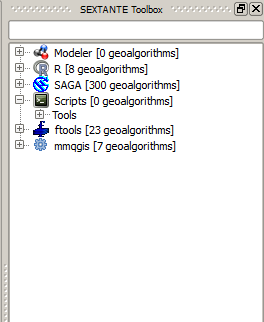
\includegraphics[width=.5\columnwidth]{toolbox.png}
\end{center}

The toolbox contains all the algorithms available, divided into groups. Each group represents a so--called algorithm provider, which is a set of algorithms coming from the same source, for instance, from a third--party application with geoprocessing capabilities. Some of this groups represent algorithms from one of such third--party applications (currently, SAGA and R), while other contain algorithms directly coded along with SEXTANTE elements, not relying on any additional software. Currently, these providers all reuse code from already--existing QGIS plugins (more specifically, from the fTools vector library shiped along with QGIS and the contributed mmqgis plugin that you can install using the plugin manager), making them more useful, since they can be executed from elements such as the modeler or the batch processing interface, which we will soon describe.

Additionaly, two more providers can be found, namely ``Models'' and ``Scripts''. This providers include user--created algorithms, and allow you to define your own workflows and processing tasks. We will devote a full chapter to each one of them a bit later.

In the upper part of the toolbox you can find a text box. To reduce the number of algorithms shown in the toolbox and make it easier to find the one you need, you can enter any word or phrase on the text box. Notice that, as you type, the number of algorithms in the toolbox is reduced to just those which contain the text you have entered in their names.

To execute an algorithm, just double--click on its name in the toolbox.

\section{The algorithm dialog}

Once you double--click on the name of the algorithm that you want to execute, a dialog similar to the next one is shown (in this case, the dialog corresponds to the \emph{SAGA--Convergence index} algorithm).

\begin{center}
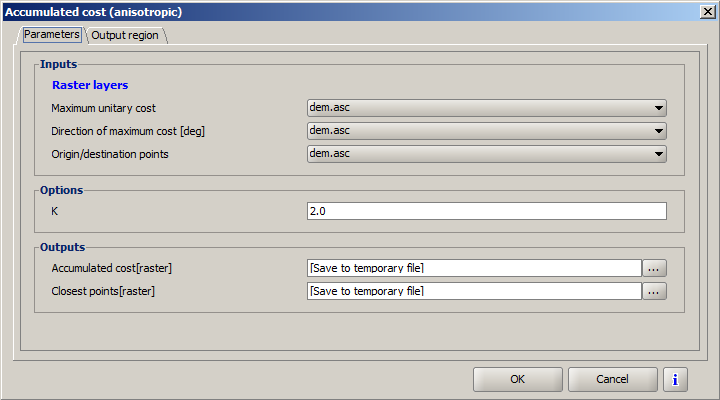
\includegraphics[width=.8\columnwidth]{accumulated_cost_anisotropic.png}
\end{center}

This dialog is used to set the input values that the algorithm needs to be executed. It shows a table where input values and configuration parameters are to be set. It, of course, has a different content depending on the requirements of the algorithm to be executed, and is created automatically based on those requirements. On the left side, the name of the parameter is shown. On the right side the value of the parameter can be set.

Although the number and type of parameters depend on the characteristics of the algorithm, the structure is similar for all of them. The parameters found on the table can be of one of the following types.

\begin{itemize}
	\item A raster layer, to select from a list of all the ones available (currently opened) in QGIS
	\item A vector layer, to select from a list of all the ones available in the QGIS
	\item A table, to select from a list of all the ones available in QGIS
	\item An option, to choose from a selection list of possible options
	\item A numerical value, to be introduced in a text box. 
	\item A range, with min and max values to be introduced in two text boxes
	\item A text string, to be introduced in a text box
	\item A field, to choose from the attributes table of a vector layer or a single table selected in another parameter.
	\item A list of elements (whether raster layers, vector ones or tables), to select from the list of the ones available in QGIS. To make the selection, click on the small button on the left side of the corresponding row to see a dialog like the following one.
		\begin{center}
		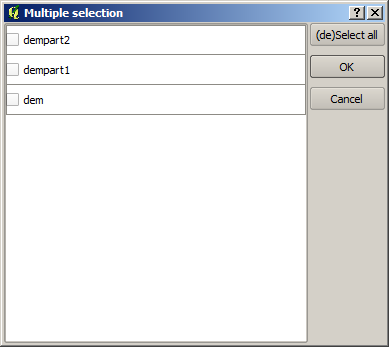
\includegraphics[width=.4\columnwidth]{multiple_selection.png}
		\end{center}		
	\item A small table to be edited by the user. These are used to define parameters like lookup tables or convolution kernels, among others.

	Click on the button on the right side to see the table and edit its values. 
\begin{center}
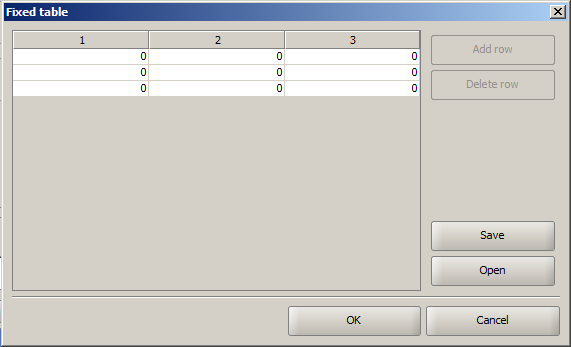
\includegraphics[width=.8\columnwidth]{fixed_table.png}
\end{center}

Depending on the algorithm, the number of rows can be modified or not, using the buttons on the right side of the window.

\end{itemize}

\section{Data objects generated by SEXTANTE algorithms}

Data objects generated by SEXTANTE can be of any of the following types:

\begin{itemize}
 \item A raster layer
\item A vector layer
\item A table
\item An HTML file (used for text and graphical outputs)
\end{itemize}

They are all saved to disk (there are no in--memory results), and the parameters table will contain a text box corresponding to each one of these outputs, where you can type the output channel to use for saving it. An output channel contains the information needed to save the resulting object somewhere. In the most usual case, you will save it to a file, but the architecture of SEXTANTE allows for any other way of storing it. For instance, a vector layer can be stored in a database or even uploaded to a remote server using a WFS--T service. Although solutions like these are not yet implemented, SEXTANTE is prepared to handle them, and we expect to add new kinds of output channels in a near feature.



%\begin{center}
%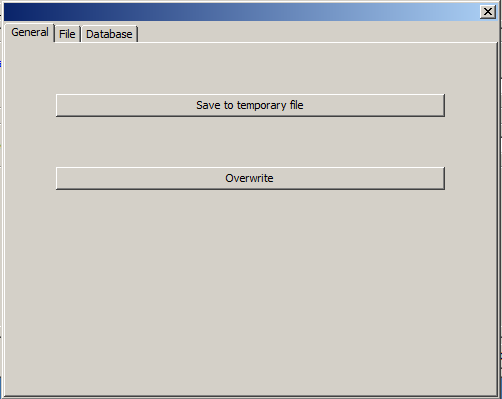
\includegraphics[width=.7\columnwidth]{output_channels.png}
%\end{center}

To select an output channel, just click on the button on the right side of the text box. That will open a save fiel dialog, where you can select the desired file path. Supported file extensions are shown in the file format selector of the dialog, depending on the kind of output and the algorithm.

The format of the output is defined by the filename extension. The supported formats depend on the ones supported by the algorithm itself. To select a format, just select the corresponding file extension (or add it if you are directly typing the filepath instead). If the extension of the filepath you entered does not match any of the supported ones, a default extension (usually dbf for tables, tif for raster layers and shp for vector ones) will be appended to the filepath and the file format corresponding to that extension will be used to save the layer or table.

If you do not enter any filename, result will be saved as temporary files and in the corresponding default file format, and will be deleted once you exit QGIS (take care with that in case you save your project and it contains temporary layers)

You can set a default folder for output data objects. Go to the configuration dialog (you can open it from the SEXTANTE menu), and in the ``General'' group you will find a parameter named ``Output folder''. This output folder is used as the default path in case you type just a filename with no path (i.e. \texttt{myfile.shp}) when executing an algorithm. 

Apart from raster layers and tables, SEXTANTE also generates graphics and texts as HTML files. These results are shown at the end of the algorithm execution in a new dialog. This dialog will keep the results produced by SEXTANTE during the current session, and can be shown at any time by selecting the \emph{SEXTANTE Results} menu.

\section{Configuring SEXTANTE}

As it has been mentioned, the configuration menu gives access to a new dialog where you can configure how SEXTANTE works. Configuration parameters are structured in separate blocks that you can select on the left--hand side of the dialog.

Apart from the ``General'' block, with the aforementioned ``Output folder'' entry, you will find one for each algorithm provider. They contain an ``Activate'' item that you can use to make algorithm appear or not in the toolbox. Also, some algorithm providers have their own configuration items, that we will explain later when covering particular algorithm providers.
